\documentclass{VUMIFPSmagistrinis}
\usepackage{algorithmicx}
\usepackage{algorithm}
\usepackage{algpseudocode}
\usepackage{amsfonts}
\usepackage{amsmath}
\usepackage{bm}
\usepackage{caption}
\usepackage{color}
\usepackage{float}
\usepackage{graphicx}
\usepackage{listings}
\usepackage{subfig}
\usepackage{wrapfig}


\university{Vilniaus universitetas}
\faculty{Matematikos ir informatikos fakultetas}
\department{Informatikos institutas}
\papertype{Programų sistemų architektūros ir projektavimo laboratorinis darbas}
\title{Architektūriniai požiūriai}
\titleineng{Architectural viewpoints}
\author{Matas Savickis}
\reviewer{}

\supervisor{Rimantas Kybartas, Partn. Prof., Dr.}

\date{Vilnius – \the\year}

\bibliography{bibliografija}

\begin{document}
\maketitle

\tableofcontents
	\section{Sistema}
		Žmonės turi daiktų, kuriuos nori parduoti, tačiau nežino kiek tiksliai jų parduodamas daiktas gali būti vertas.
		Sistema leidžia vartotojams parduoti daiktus aukciono principu.
		Vartotojas įdeda norimą daiktą į aukcioną nustatydamas mažiausią kainą už kurią sutiktų parduoti daiktą, nustato aukciono trukmę ir kiti sistemos parduotojai gali didinti daikto kainą iki nustatyto laiko.
		Sistema suteikia galimybę atsiskaityti už prekes elektroninio banko pervedimais ir kriptovaliutomis.
	\section{Suinteresuoti asmenys}
		\begin{itemize}
			\item{Pirkėjai - vartotojai, kurie naudosis aukcionu siekdami parduoti prekę.}
			\item{Pardavėjai - vartotojai, kurie naudosis aukcionu siekdami nusipirkti prekę.}
			\item{Investuotojai - žmonės, kurie rems projekto įgyvendinimą finansiškai}
			\item{Programuotojai - žmonės, kurie kurs sistemą.}
			\item{Testuotojai - žmonės, kurie testuos sistemą.}
			\item{Policija - suinteresuota nelegalių daiktų pirkėjų ir pardavėjų identifikavimu.}
			\item{Lietuvos teismas - suinteresuotas nelegalių prekių pirkimu ir pardavimu, taip pat Lietuvos įstatymų laikymusi.}
			\item{Europos sąjunga - suinteresuota, kad sistema laikytusi europos sąjungos įstatymų ir reglamentų(BDAR)}
		\end{itemize}
		\section{Konteksto požiūrio taškas}
			\subsection{Sistemos taikymo sritis}
				Vartotojas sistemoje įkelią savo skelbimą, kiti vartotojai dalyvauja aukcione ir didžiausią kainą pasiūlęs vartotojas laimi aukcioną.
				Aukcioną laimėjęs žmogus perveda pinigus arba Bitcoin kripto valiutą į mūsų sistema, tuomet prekės pardavėjas išsiunčia prekę į mūsų biurą patikrinti ar prekė atitinka aprašymą. 
				Biuro darbuotojui patvirtinus, kad prekė atitinka aprašymą sistema perveda pinigus pardavėjui jo pasirinktu būdu.

			\subsection{Konteksto požiūrio taško diagrama}

				\begin{figure}[H]
				\centering
				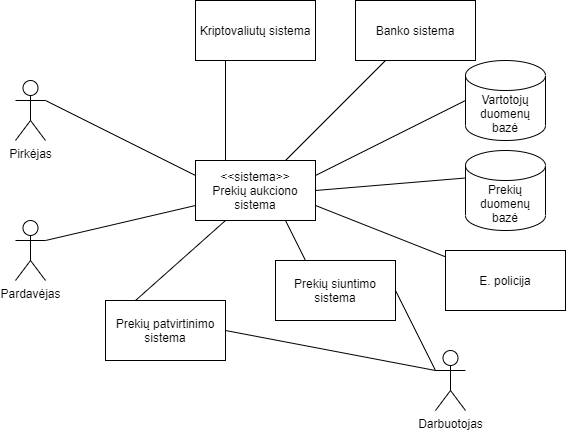
\includegraphics[scale=0.9]{img/context}
				\caption{Aukciono sistemos konteksto požiūrio taško diagrama} % Antraštė įterpiama po paveikslėlio
				\label{img:text}
				\end{figure}
	
			\subsection{Funkciniai reikalavimai}
				\subsubsection{Pardavėjas reikalavimai}
					\begin{enumerate}
						\item{Pirkėjas turi galimybę įdėti prekę į aukcioną nurodydamas jos pradinę kainą, aukciono trukmę, aprašymą ir įkeldamas fotogtafiją.}
						\item{Pirkėjas atšaukti aukcioną jam nepasibaigus taip nebeparduodant prekės.}
						\item{Atsiradus pirkėjui, po aukciono pardavėjas turi prekę išsiųsti į aukciono sandelį per dvi darbo dienas.}
						\item{Pirkėjas pardavęs prekę gali pasirinkti išmokėjimo būdą: pavedimas į sąskaitą, kriptovaliutas, aukciono sąskaitos papildymas.}
					\end{enumerate}
				\subsubsection{Pirkėjas reikalavimai}
					\begin{enumerate}
						\item{Pirkėjas norėdamas dalyvauti aukcione turi įsidėti pinigų į aukciono sąskaitą.}
						\item{Aukciono sąskaitą galima papildyti per elektroninį banką arba pervedant kripto valiutas į sistemos piniginę.}
						\item{Pirkėjas gali siūlyti didesnę prekės kainą kol prekės aukcionas nepasibaigė.}
						\item{Paskutinis aukščiausią kainą pasiūlęs pirkėjas laimi aukcioną.}
						\item{Aukciono nugalėtojas gali sekti jam atkeliaujančia prekę.}
						\item{Nugalėtojui negavus prekės jo pinigai pervedami į aukciono sąskaitą.}
						\item{Pirkėjas gali komentuoti prie kiekvienos prekės.}
						\item{Pirkėjas gali persivesti savo aukciono sąskaitą į savo kriptovaliutų piniginę arba į savo bankinę sąskaitą.}
					\end{enumerate}
				\subsubsection{Prekių siuntimo reikalavimai}
					\begin{enumerate}
						\item{Pardavėjui atsiuntus prekę į aukciono sandėlį prekė yra patvirtinama aukciono darbuotojo ar siuntinys atitinka aukcione pateiktą prekės aprašymą ir nuotrauką.}
						\item{Gavus įtartiną siuntinį aukciono darbuotojas informuoja policiją pateikdamas pirkėjo ir pardavėjo duomenis}
						\item{Jeigu prekė neatitinka aprašymo ir fotografijos pinigai būna gražinami pirkėjui ir krepė yra išsiunčiama pardavėjui išperkamosios siuntos principu.}
					\end{enumerate}
				\subsubsection{Banko reikalavimai}
					\begin{enumerate}
						\item{Sistemoje yra galimybė pervesti pinigus iš banko sąskaitos į aukciono sąskaitą.}
						\item{Sistemoje yra galimybę gauti pinigus iš aukciono sąskaitos į banko sąskaitą.}
						\item{Bankinės pranzakcijos yra vykdomos banklink paslauga.}
					\end{enumerate}
				\subsubsection{Kriptovaliutų reikalavimai}
					\begin{enumerate}
						\item{Sistemoje yra galimybė pervesti kritovaliutas iš kripto piniginės į aukciono sąskaitą, kripto valiutos automatiškai konvertuojamos į eurus taikant papildoma mokestį. }
						\item{Sistemoje yra galimybė pervesti pinigus iš aukciono sąskaitos į kriptovaliutų piniginę taikant papildomą mokestį.}
					\end{enumerate}
				\subsubsection{Policijos reikalavimai}
					\begin{enumerate}
						\item{Policijai apie nelegalias prekes yra pranešama naudojanti e. Policija paslaugomis.}
					\end{enumerate}
				\subsubsection{Teisiniai reikalavimai}
					\begin{enumerate}
						\item{Sistema veikia laikydamasi Lietuvos įstatymų.}
						\item{Sistema veikia laikydamasi Europos įstatymų ir BDAR reglamento.}
					\end{enumerate}
				\subsubsection{Bendri reikalavimai}
					\begin{enumerate}
						\item{Vartotojui paprašius jo duomenys yra pašalinami iš sistemos per mėnesį.}
						\item{Vartotojas gali matyti savo pirkimų ir pardavimų istoriją.}	
					\end{enumerate}
			
		\section{Funkcinis požiūrio taškas}
		\section{Informacijos požiūrio taškas}
		\section{Lygiagretumo požiūrio taškas}
		\section{Kūrimo požiūrio taškas}
		\section{Diegimo požiūrio taškas}
		\section{Operatyvinis požiūrio taškas}
		


\end{document}
